\documentclass{article}
\usepackage{../../Self_Style}

\title{Phys 20AL Week 5: Waves on a string}
\author{Zih-Yu Hsieh}
\date{\today}

\begin{document}
\maketitle

\section{Aim for the Experiment}
The goal is to figure out the relationship between the velocity of wave propogation, and its tension force. It is also aimed to figure out the coefficient $\mu$ - the mass per unit length of the string - based on the measured data.

\hfil

\section{Experimental Setup}
\subsection{Experiment with Manual Setup}
The equipments include: Tape, Long string, meter stick, mass, mass scale, pully, phone (with slow-motion camera).

The setup process is as follow:
\begin{itemize}
    \item[1.] Fix the pully at the edge of the table. 
    \item[2.] Tape one end of the string on the wall, and put the other end on the pully.
    \item[3.] Hang suitable mass onto the string at the end of the pully.
\end{itemize}

\subsection{Experiment with Function Generator}
The equipments include: String, meter stick, masses, mass scale, pully, function generator, string vibrator.

The setup process is as follow:
\begin{itemize}
    \item[1.] Plugin the function generator's power chord, and connect the string vibrator to the function generator.
    \item[2.] Fix both the pully and the string vibrator at the edge of the table, with suitable distance in between.
    \item[3.] Tie one end of the string on the string vibrator, and put the other end on the pully.
\end{itemize}

\hfil

\section{Measurement and Methods of Measure}
The length of the string will be measured using meter stick, the masses about to hang on the string (to generate steady tension force on the string). About the wave velocity, there are two types:
\begin{itemize}
    \item For the one with anual measurement, the time for the wave propogation is measured using the camera recording (for more accuracy it's intended to use slow-motion mode in the camera).
    \item For the one with function generator, instead of measuring the time for the wave propogation, it's measuring the frequency of the string oscillation generated by the Function Generator.
\end{itemize}

\textbf{Thought:} The use of the pully is to direct the string downward, so it directly transfers the force of gravity on the masses into the tension force of the string.

\hfill

For each of the case, the masses measured and used are as below:
\begin{itemize}
    \item[1.] For experiment that measures everything manually, the mass is $0.025$ kg.
    \item[2.] For experiment that measures the first resonance frequencey with varying masses, the masses used include: $0.055,0.105,0.160,0.205,0.255,0.306$ kg.
    \item[3.] For the experiment that measures multiple resonance frequencies of the same masses, the masses used include: $0.100, 0.200$ kg.  
\end{itemize}

For each of the case, the string length used are as below:
\begin{itemize}
    \item For experiment that measures everything manually, the string length is $6.000$ m.
    \item For both experiments with function generator, the string length is $0.865$ m.
\end{itemize}

\hfil

For the first experiment that measures everything manually, we'll do a total of $3$ trials to measure the velocity of the wave propogation.

For the second experiment using function generator and measuring first resonance for varying masses, each chosen mass will also do a total of $3$ trials to measure the first resonance frequency. (the idea is to get more experimental data of the overall first resonance frequency).

For the third experiment however, instead of measuring with multiple trials, for each mass we'll perform 1 measurement at each resonance frequency, until it is no longer observable. (This typically happens around the $n^\textmd{th}$ resonance frequency, where $n=6,7$).

\hfil

\section{Experimental Procedure}
\subsection{Experiment with Manual Setup}
The goal for this section is to get a rough / general observation about the wave propogation, instead of performing a precise measurement.

We'll follow the following procedure:
\begin{itemize}
    \item[1.] Measure the mass used for tension, and hang the mass at the end of the string that's at the pully's side.
    \item[2.] Gently tap the string on the other end (that is taped), but with large enough amplitude that can be observed and recorded by the camera.
    \item[3.] For the whole process in Step 2, record using the slow-motion camera till the time that the wave has traveled back to the initial starting point.
    \item[4.] Repeat step 2 to 3 for the total of 3 times.   
\end{itemize}

\subsection{Experiment with Function Generator}
\subsubsection{Experiment Measuring 1st Resonance Frequency}
The goal for this section is to derive the velocity of the wave using the resonance frequency, and further derive the string's mass per unit length constant $\mu$ using the known velocity and tension.

We'll follow the following procedure:
\begin{itemize}
    \item[1.] Fix a mass used for tension, measure the mass, and hang it at the end of the string (on the pully's side).
    \item[2.] Start the function generator, and let the string vibrator vibrate the string.
    \item[3.] Tweak the output frequency on the function generator, until the first resonance is observed (which requires the string to have stable amplitude, and the pully is not oscillating back and forth; or more precisely, when the string has a fixed point at the end). Record this first resonance frequency displayed on the function generator.
    \item[4.] Repeat Step 2 to 3 for a total of 3 trials for the fixed mass.
    \item[5.] Change the mass mentioned in Step 1, and repeat Step 2 to 4 for each desired mass.
\end{itemize}

\subsubsection{Experiment Measuring nth Resonance Frequency}
The goal for this section is to observe multiple resonance frequency when fixing a specific tension force, observe the change of wavelength under different frequencies, and also see if the wave velocity is independent from the resonance frequency (when fixing tension).

We'll follow the following procedure:
\begin{itemize}
    \item[1.] Fix a mass used for tension, measure the mass, and hang it at the end of the string (on the pully's side).
    \item[2.] Start the function generator, and let the string vibrator vibrate the string.
    \item[3.] Tweak the output frequency on the function generator, until the first resonance is observed (which requires the string to have stable amplitude, and the pully is not oscillating back and forth; or more precisely, when the string has a fixed point at the end). Record this first resonance frequency displayed on the function generator.
    \item[4.] Repeat Step 3 inductively for each $n^\textmd{th}$ resonance frequency (for $n=2,3,...$) until the resonance is no longer observable.
    \item[5.] Change the masses to other ones await to be measured, and repeat Step 2 to 4 for the desired mass.
\end{itemize}

\hfil

\section{Experimental Data}
\subsection{Experiment with Manual Setup}
\begin{figure}[h!]
    \centering
    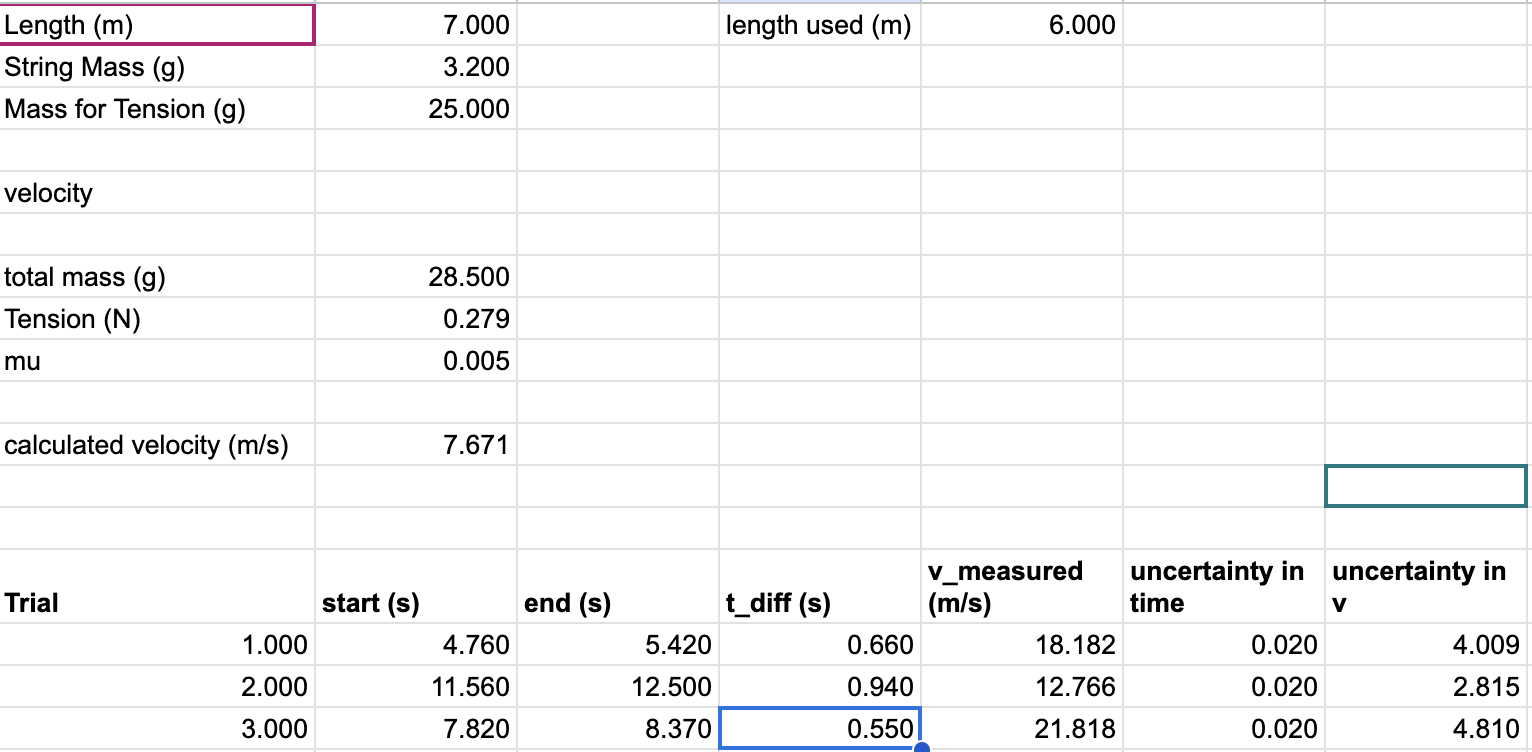
\includegraphics[width=150mm]{data_manual.png}
\end{figure}

\subsection{Experiment with Function Generator}
\subsubsection{Experiment Measuring 1st Resonance Frequency}
\begin{figure}[h!]
    \centering
    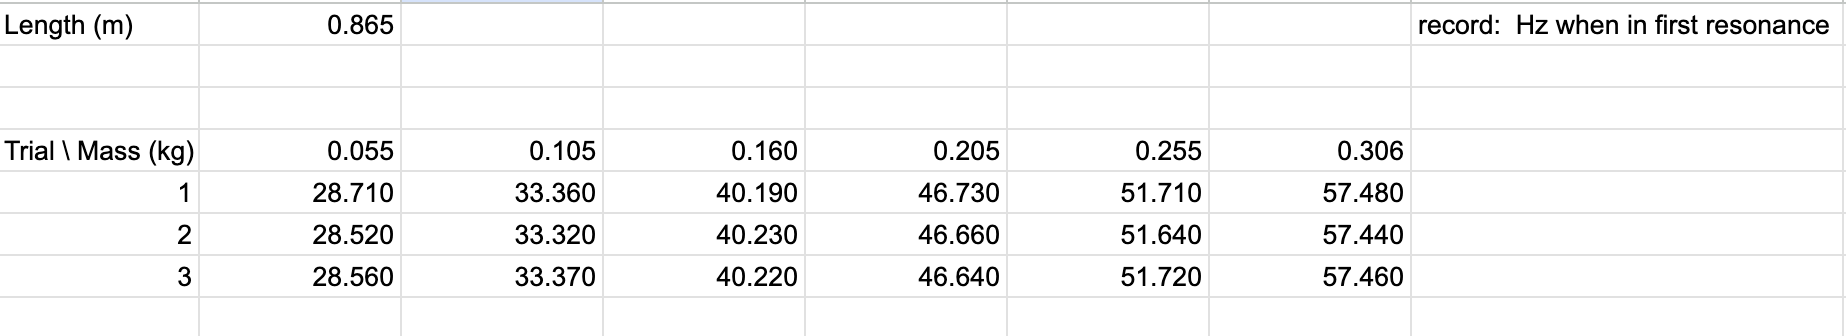
\includegraphics[width=150mm]{data_device_1.png}
\end{figure}
\subsubsection{Experiment Measuring nth Resonance Frequency}
\begin{figure}[h!]
    \centering
    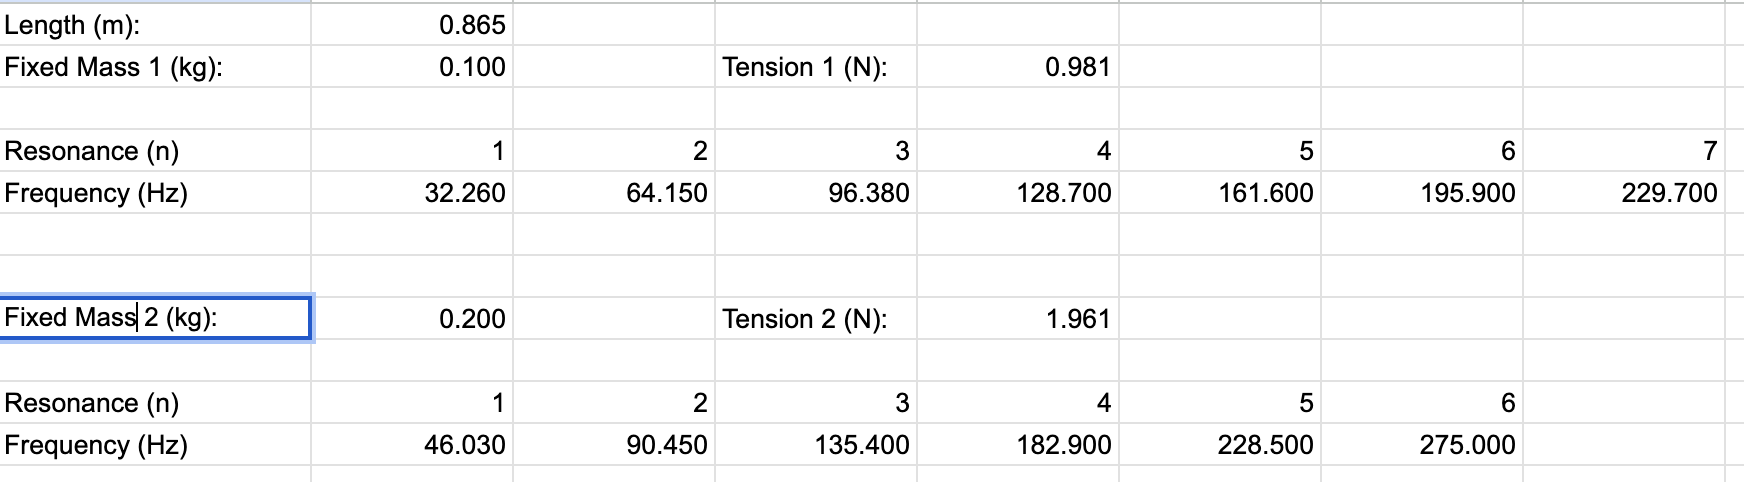
\includegraphics[width=150mm]{data_device_2.png}
\end{figure}

\newpage

\end{document}